\section{Submitter}

\begin{figure}[H]
    \centering
    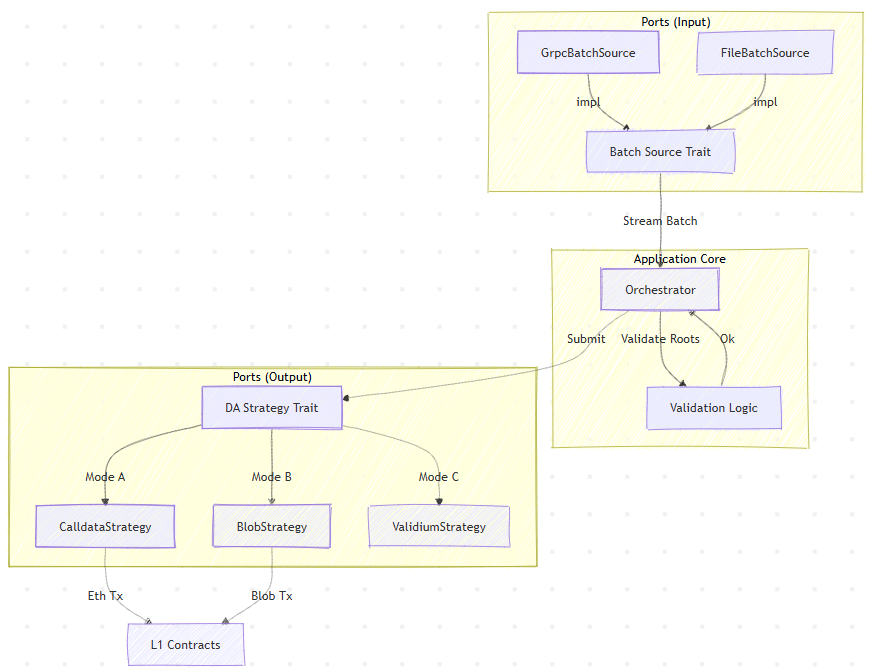
\includegraphics[width=0.90\textwidth]{figures/chapter4/submitter_arch.png}
    \caption{Submitter Component Architecture.}
    \label{fig:submitter_arch}
\end{figure}

\label{sec:submitter}
The Submitter acts as the bridge relayer, reliably pushing executed batch data from Layer-2 back to the Layer-1 Ethereum network.

\begin{itemize}
    \item \textbf{Language:} Rust.
    \item \textbf{Workflow (Saga Engine):} Subscribes to the Executor stream via a gRPC Client (compiled using \texttt{protobuf-compiler}). To ensure reliable interaction with the L1 network despite potential node disconnections or nonce desynchronization, the Submitter utilizes a Saga Workflow Engine. This state machine, backed by a persistent database, manages reliable retries, idempotency guarantees, and complex error recovery for L1 RPC calls.
    \item \textbf{Data Availability Formatter:} The DA Formatter is responsible for structuring the execution payload according to the configured DA mode before submission. Crucially, it supports encoding state diffs into standard \texttt{Calldata} or generating the necessary KZG commitments for \texttt{EIP-4844 Blob} data representations. Off-chain DA is implemented only as a local simulated stub.
    \item \textbf{Output:} Broadcasts transactions to the L1 Hardhat node via \texttt{eth\_sendRawTransaction} and records critical latency and gas metrics to \texttt{submitter\_metrics.json}.
\end{itemize}

As depicted in Figure~\ref{fig:submitter_arch}, the Submitter component interacts with the L1 smart contracts to finalize transaction batches.
